\documentclass[tikz,border=10pt]{standalone}
\usetikzlibrary{arrows.meta, positioning, calc, decorations.pathreplacing}
\usepackage{amsmath}
\usepackage{amssymb}

\begin{document}
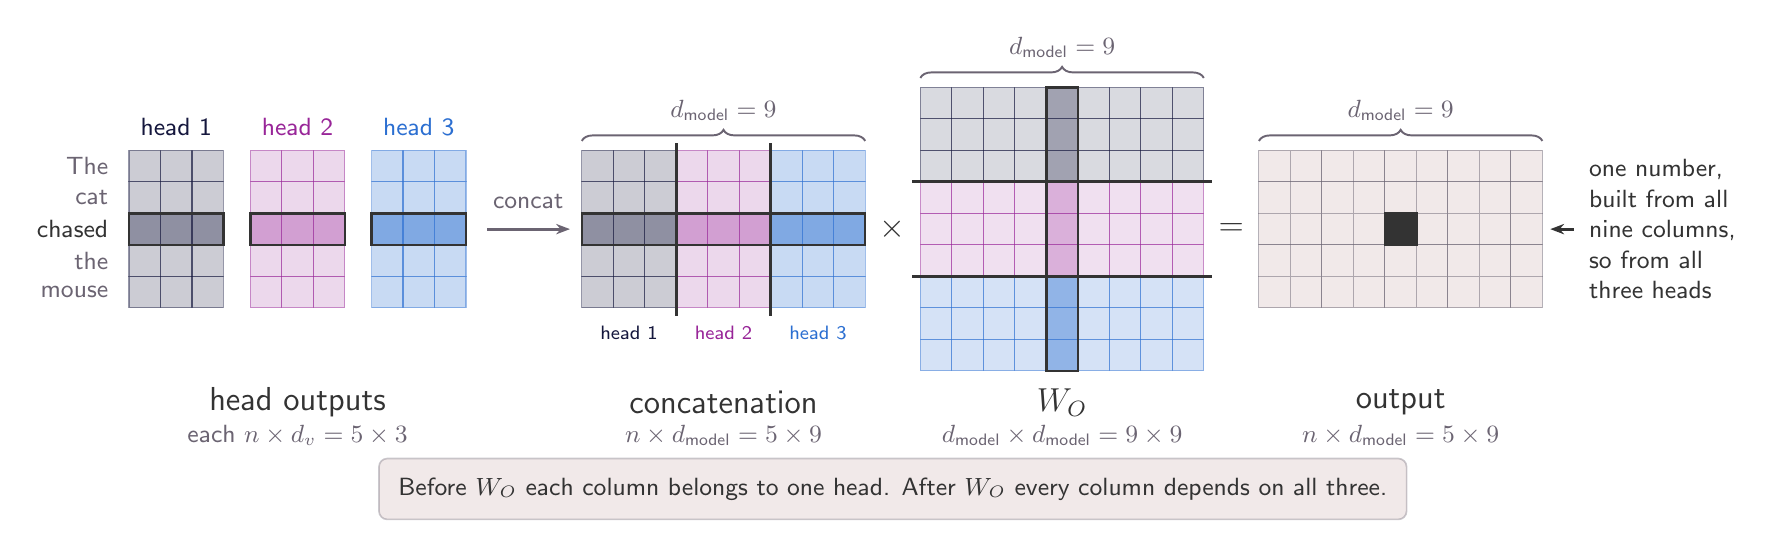
\begin{tikzpicture}[
    every node/.style={font=\sffamily},
]

\definecolor{c1}{HTML}{15173D}   % head 1
\definecolor{c2}{HTML}{982598}   % head 2
\definecolor{c3}{HTML}{E491C9}
\definecolor{head3}{HTML}{2C6FD1}  % head 3, a blue distinct from c1 navy
\definecolor{c4}{HTML}{F1E9E9}
\definecolor{axiscolor}{HTML}{333333}
\definecolor{labelcolor}{HTML}{6B6472}

\def\cs{0.40}    % cell size, shared by every matrix here

% ================================================================
%  Everything is centred on the line y = 0.
%
%  head 1 / 2 / 3   5 x 3   top y = 1.00,  x0 = 0.00 / 1.54 / 3.08
%  concat           5 x 9   top y = 1.00,  x0 = 5.75   (-> 9.35)
%  W_O              9 x 9   top y = 1.80,  x0 = 10.05  (-> 13.65)
%  output           5 x 9   top y = 1.00,  x0 = 14.35  (-> 17.95)
%
%  row r spans y in [top - (r+1)cs, top - r cs]
%  col c spans x in [x0 + c cs, x0 + (c+1) cs]
%
%  The trace:  row 2 (chased) of the concat  x  column 4 of W_O
%              = the single dark cell at row 2, column 4 of the output.
%  Row 2 of the concat sits at y in [-0.20, 0.20]; column 4 of W_O at
%  x in [11.65, 12.05]; both cross the centre line, so the three
%  highlights land at the same height and read as one path.
%
%  Block boundaries: vertical rules in the concat at x = 6.95, 8.15;
%  horizontal rules in W_O at y = 0.60, -0.60. Same rule, same meaning:
%  column block j of the concat meets row block j of W_O.
%
%  y = 1.30   head labels
%  y = 1.12 / 1.92 column braces (concat / W_O)
%  y = -1.32  the three block labels under the concat
%  y = -2.20  matrix names,  y = -2.62 shapes
%  y = -3.15  the takeaway panel
% ================================================================

% ---------------------------------------------------------------- head outputs
\foreach \hc/\hop/\hhi/\i/\n in {c1/0.22/0.48/0/1, c2/0.18/0.44/1/2, head3/0.26/0.60/2/3} {
    \foreach \r in {0,...,4} {
        \foreach \c in {0,1,2} {
            \pgfmathsetmacro{\op}{ifthenelse(\r==2, \hhi, \hop)}
            \fill[\hc, opacity=\op]
                (\i*1.54+\c*\cs, 1.00-\r*\cs-\cs) rectangle ++(\cs, \cs);
            \draw[\hc, opacity=0.45, line width=0.4pt]
                (\i*1.54+\c*\cs, 1.00-\r*\cs-\cs) rectangle ++(\cs, \cs);
        }
    }
    % chased's row, the one followed all the way across the figure
    \draw[axiscolor, line width=0.9pt] (\i*1.54, -0.20) rectangle ++(1.20, 0.40);
    \node[font=\sffamily\small, text=\hc] at (\i*1.54+0.60, 1.30) {head \n};
}

\foreach \w/\r in {The/0, cat/1, the/3, mouse/4} {
    \node[font=\sffamily\small, text=labelcolor, anchor=east]
        at (-0.14, 1.00-\r*\cs-0.5*\cs) {\w};
}
\node[font=\sffamily\small, text=axiscolor, anchor=east] at (-0.14, 0) {chased};

\node[font=\sffamily\large, text=axiscolor] at (2.14, -2.20) {head outputs};
\node[font=\sffamily\small, text=labelcolor] at (2.14, -2.62)
    {each $n \times d_v = 5 \times 3$};

% ---------------------------------------------------------------- concat arrow
\draw[-{Stealth[length=5pt]}, line width=1.0pt, labelcolor] (4.55, 0) -- (5.60, 0);
\node[font=\sffamily\small, text=labelcolor, anchor=south] at (5.07, 0.14)
    {concat};

% ---------------------------------------------------------------- concatenation
\foreach \hc/\hop/\hhi/\i in {c1/0.22/0.48/0, c2/0.18/0.44/1, head3/0.26/0.60/2} {
    \foreach \r in {0,...,4} {
        \foreach \cc in {0,1,2} {
            \pgfmathsetmacro{\c}{\i*3+\cc}
            \pgfmathsetmacro{\op}{ifthenelse(\r==2, \hhi, \hop)}
            \fill[\hc, opacity=\op]
                (5.75+\c*\cs, 1.00-\r*\cs-\cs) rectangle ++(\cs, \cs);
            \draw[\hc, opacity=0.45, line width=0.4pt]
                (5.75+\c*\cs, 1.00-\r*\cs-\cs) rectangle ++(\cs, \cs);
        }
    }
    \node[font=\sffamily\scriptsize, text=\hc] at (5.75+\i*1.20+0.60, -1.32)
        {head \the\numexpr\i+1\relax};
}
% the blocks have not mixed: a hard boundary at columns 3|4 and 6|7
\draw[axiscolor, line width=1.0pt] (6.95, -1.10) -- (6.95, 1.10);
\draw[axiscolor, line width=1.0pt] (8.15, -1.10) -- (8.15, 1.10);
% chased's row, now nine numbers wide
\draw[axiscolor, line width=0.9pt] (5.75, -0.20) rectangle ++(3.60, 0.40);

\draw[decorate, decoration={brace, amplitude=4pt}, labelcolor, line width=0.7pt]
    (5.75, 1.12) -- (9.35, 1.12);
\node[font=\sffamily\small, text=labelcolor, anchor=south] at (7.55, 1.26)
    {$d_{\text{model}} = 9$};

\node[font=\sffamily\large, text=axiscolor] at (7.55, -2.20) {concatenation};
\node[font=\sffamily\small, text=labelcolor] at (7.55, -2.62)
    {$n \times d_{\text{model}} = 5 \times 9$};

\node[font=\sffamily\large, text=axiscolor] at (9.70, 0) {$\times$};

% ---------------------------------------------------------------- W_O
\foreach \hc/\hop/\hhi/\i in {c1/0.16/0.40/0, c2/0.14/0.36/1, head3/0.20/0.52/2} {
    \foreach \rr in {0,1,2} {
        \foreach \c in {0,...,8} {
            \pgfmathsetmacro{\r}{\i*3+\rr}
            \pgfmathsetmacro{\op}{ifthenelse(\c==4, \hhi, \hop)}
            \fill[\hc, opacity=\op]
                (10.05+\c*\cs, 1.80-\r*\cs-\cs) rectangle ++(\cs, \cs);
            \draw[\hc, opacity=0.45, line width=0.4pt]
                (10.05+\c*\cs, 1.80-\r*\cs-\cs) rectangle ++(\cs, \cs);
        }
    }
}
% the same boundary as in the concat, turned on its side
\draw[axiscolor, line width=1.0pt] (9.95, 0.60) -- (13.75, 0.60);
\draw[axiscolor, line width=1.0pt] (9.95, -0.60) -- (13.75, -0.60);
% one column of W_O, which runs through all three row blocks
\draw[axiscolor, line width=0.9pt] (11.65, -1.80) rectangle ++(0.40, 3.60);

\draw[decorate, decoration={brace, amplitude=4pt}, labelcolor, line width=0.7pt]
    (10.05, 1.92) -- (13.65, 1.92);
\node[font=\sffamily\small, text=labelcolor, anchor=south] at (11.85, 2.06)
    {$d_{\text{model}} = 9$};

\node[font=\sffamily\large, text=axiscolor] at (11.85, -2.20) {$W_O$};
\node[font=\sffamily\small, text=labelcolor] at (11.85, -2.62)
    {$d_{\text{model}} \times d_{\text{model}} = 9 \times 9$};

\node[font=\sffamily\large, text=axiscolor] at (14.00, 0) {$=$};

% ---------------------------------------------------------------- output
\foreach \r in {0,...,4} {
    \foreach \c in {0,...,8} {
        \ifnum\r=2 \ifnum\c=4 \colorlet{outfill}{axiscolor}\else
            \colorlet{outfill}{c4}\fi \else \colorlet{outfill}{c4}\fi
        \fill[outfill] (14.35+\c*\cs, 1.00-\r*\cs-\cs) rectangle ++(\cs, \cs);
        \draw[labelcolor, opacity=0.5, line width=0.4pt]
            (14.35+\c*\cs, 1.00-\r*\cs-\cs) rectangle ++(\cs, \cs);
    }
}
\draw[axiscolor, line width=0.9pt] (15.95, -0.20) rectangle ++(0.40, 0.40);

\draw[decorate, decoration={brace, amplitude=4pt}, labelcolor, line width=0.7pt]
    (14.35, 1.12) -- (17.95, 1.12);
\node[font=\sffamily\small, text=labelcolor, anchor=south] at (16.15, 1.26)
    {$d_{\text{model}} = 9$};

\node[font=\sffamily\large, text=axiscolor] at (16.15, -2.20) {output};
\node[font=\sffamily\small, text=labelcolor] at (16.15, -2.62)
    {$n \times d_{\text{model}} = 5 \times 9$};

% ---------------------------------------------------------------- the one cell
\draw[-{Stealth[length=5pt]}, line width=1.0pt, axiscolor] (18.35, 0) -- (18.05, 0);
\node[font=\sffamily\small, text=axiscolor, anchor=west, align=left]
    at (18.42, 0) {one number,\\built from all\\nine columns,\\so from all\\three heads};

% ---------------------------------------------------------------- takeaway
\node[font=\sffamily\small, text=axiscolor, anchor=center, align=center,
      fill=c4, draw=labelcolor, draw opacity=0.35, line width=0.6pt,
      rounded corners=3pt, inner sep=7pt]
    at (9.70, -3.30)
    {Before $W_O$ each column belongs to one head.
     After $W_O$ every column depends on all three.};

\end{tikzpicture}
\end{document}
